\documentclass[11pt,a4paper]{article}

% --- Packages ---
\usepackage[utf8]{inputenc}
\usepackage[T1]{fontenc}
\usepackage{lmodern}
\usepackage[margin=2.5cm]{geometry}
\usepackage{amsmath,amssymb}
\usepackage{graphicx}
\usepackage{booktabs}
\usepackage{multirow}
\usepackage{tabularx}
\usepackage{float}
\usepackage[labelfont=bf,font=small]{caption}
\usepackage{enumitem}
\usepackage[hidelinks]{hyperref}
\usepackage{natbib}
\bibliographystyle{apalike}
\usepackage{xcolor}
\usepackage{url}

% compact lists
\setlist{nosep}

\title{Cognitive-Linguistic Network Structure of OCD Personal Narratives:\\
A Three-Group Comparison Using TEA Networks\\and Recurrence Quantification Analysis}

\author{
Jacopo Schenetti\\
\textit{University of Trento}\\
\texttt{jacopo.schenetti@studenti.unitn.it}
}

\date{}

\begin{document}
\maketitle

% =====================================================================
\begin{abstract}
Personal narratives encode cognitive patterns that vary across mental health conditions, but few studies have compared how different disorders shape the structure of self-narration. This study uses two computational methods, Target-Event-Agent (TEA) cognitive networks and Recurrence Quantification Analysis (RQA), to compare personal narratives of obsessive-compulsive disorder (OCD) with those of physical illness (cancer) and other mental health conditions (depression/PTSD). We analyzed 152 OCD recovery stories from a blog, 152 cancer patient stories from an interview-based website, and 200 depression/PTSD posts from Reddit. TEA networks, extracted with \citet{franchini2026tea}'s framework, showed that OCD narratives had higher first-person agent ratios than cancer narratives ($g = +1.37$, $p < .001$) but lower ratios than depression/PTSD narratives ($g = -0.45$, $p = .004$). RQA of sentence-level semantic embeddings revealed that OCD narratives had far higher thematic recurrence than cancer narratives (Recurrence Rate $g = +1.57$, Determinism $g = +1.19$, Laminarity $g = +1.24$; all $p < .001$), yet lower recurrence than depression/PTSD narratives ($g = -0.39$ to $-0.62$; all $p < .05$). After Benjamini-Hochberg correction, 16 of 19 originally significant effects survived at FDR $= .05$. Supplementary analyses separating depression from PTSD showed that the gradient was driven primarily by depression ($g = -0.71$, $p < .001$), with a smaller, non-significant gap for PTSD ($g = -0.32$, $p = .11$). OCD narratives thus sit between physical illness and affective disorder narratives on both self-focus and thematic repetitiveness, though the pattern is stronger for depression than for PTSD. These findings are consistent with the intrusion-driven nature of obsessive cognition, but platform and genre differences between the three corpora limit causal attribution to disorder type alone.

\medskip\noindent\textbf{Keywords:} obsessive-compulsive disorder, cognitive networks, TEA networks, recurrence quantification analysis, computational linguistics, personal narratives, mental health
\end{abstract}

% =====================================================================
\section{Introduction}

\subsection{Personal Narratives as Cognitive Windows}

When people narrate their illness experiences, they do more than report what happened. Their word choices, the agents they foreground, and the themes they return to all reflect underlying cognitive patterns \citep{pennebaker2011}. How individuals construct these accounts has been linked to their psychological adjustment \citep{frank1995}, and the linguistic features of such narratives can now be extracted at scale with computational tools.

Work on language and mental health has identified several stable associations. First-person singular pronoun use tracks with depression severity \citep{rude2004}, and thematic repetitiveness in discourse has been tied to ruminative cognitive styles \citep{nolenhoeksema2000}. Most of this work, however, has focused on single conditions or binary comparisons (clinical vs.\ healthy controls). It remains unclear how different conditions relate to each other within the broader space of illness narratives.

\subsection{OCD as a Distinct Cognitive Profile}

OCD is an interesting test case because its cognitive signature differs, in theory, from both physical illness and mood disorders. Cognitive models of OCD emphasize intrusive thoughts: unwanted, ego-dystonic mental events that cause distress through appraisal of threat and responsibility, not through mood congruence as in depression \citep{salkovskis1985,rachman1997}. People with OCD often describe their relationship with their own thoughts as adversarial; the self is narrated as under siege by its own cognition.

This theoretical picture leads to two testable predictions about narrative structure. First, OCD narratives should show higher self-focus than physical illness narratives (where the disease, rather than the self, is the main actor), but possibly lower self-focus than depression narratives (where pervasive low mood places the self at the center of everything). Second, OCD narratives should show more thematic recurrence than physical illness narratives (reflecting the repetitive quality of obsessions), but possibly different recurrence patterns from depression, where rumination may produce even broader thematic circularity.

\subsection{Computational Approaches: TEA Networks and RQA}

We used two methods that capture different aspects of narrative cognition.

\paragraph{Target-Event-Agent (TEA) Cognitive Networks.}
TEA networks \citep{franchini2026tea} extract ``who did what to whom'' from text via dependency parsing and represent the result as a directed graph with three node types: Agents (subjects), Events (verbs), and Targets (objects). Built on spaCy with coreference resolution, the framework preserves syntactic agency rather than reducing text to word frequencies. Each node receives a valence label (positive, negative, neutral) via VADER sentiment analysis \citep{hutto2014}, following the annotation scheme of Textual Forma Mentis Networks \citep{stella2020}. Structural metrics computed on these graphs (first-person agent ratio, density, LSCC fraction, clustering) quantify properties of the narrative's cognitive architecture.

\paragraph{Recurrence Quantification Analysis (RQA).}
RQA was originally developed for dynamical systems \citep{eckmann1987,webber1994} and has since been applied to text by treating sentence-embedding sequences as time series \citep{marwan2007}. A recurrence matrix records which sentence pairs exceed a cosine similarity threshold, and several metrics are derived from its structure: Recurrence Rate (RR, overall thematic repetition), Determinism (DET, predictability of thematic sequences), Laminarity (LAM, tendency to dwell on a theme), and Entropy (ENTR, complexity of recurrence patterns). These metrics can pick up repetitive thinking patterns in text.

\subsection{The Present Study}

We applied TEA networks and RQA to three groups of personal narratives: OCD stories, cancer patient stories, and depression/PTSD posts. Including both a physical illness control and a mental health control allows us to position OCD within a space defined by the physical-vs-mental and intrusion-vs-mood distinctions. We predicted that OCD narratives would fall between cancer and depression/PTSD on measures of self-focused agency and thematic recurrence.

% =====================================================================
\section{Methods}

\subsection{Corpora}

Three corpora of English-language personal narratives were assembled, each reflecting a different relationship to illness. The three corpora also differ in platform and genre (curated blog, edited interview site, social media), a limitation we address in the Discussion.

\paragraph{OCD Stories Corpus.}
153 first-person recovery narratives were collected from The OCD Stories (\url{theocdstories.com}), a curated blog where individuals describe their experience living with and recovering from OCD. One story was excluded due to extraction errors, leaving 152 texts ($M = 1{,}408$ words, $SD = 965$, $Mdn = 1{,}208$, range: 51--6,634). These are unsolicited, long-form accounts written for a peer audience.

\paragraph{Cancer Patient Stories Corpus.}
342 first-person narratives were collected from The Patient Story (\url{thepatientstory.com}), an interview-based site with cancer patients' accounts of diagnosis, treatment, and survivorship across 20 cancer types. After removing boilerplate, interviewer questions, and diagnostic fact boxes, and filtering for a minimum of 300 words, 342 stories remained ($M = 4{,}226$ words, $SD = 2{,}870$). For analysis, a random sample of 152 was drawn to match the OCD corpus size ($M = 4{,}339$ words, $SD = 2{,}614$).

\paragraph{Depression/PTSD Reddit Corpus.}
200 posts were sampled from the HuggingFace dataset \texttt{solomonk/reddit\_mental\_health\_posts}, a public collection of mental health subreddit posts. We selected posts from r/depression ($n = 83$) and r/ptsd ($n = 117$), keeping only those with $\geq$300 words after cleaning. Reddit-specific formatting (URLs, Markdown, edit notes) was stripped and post titles were prepended. The combined sample had $M = 539$ words, $SD = 269$; the two subreddits had similar word counts ($M_\mathrm{dep} = 542$, $SD_\mathrm{dep} = 286$; $M_\mathrm{ptsd} = 536$, $SD_\mathrm{ptsd} = 258$).

The three corpora differ in mean word count because of their different genres. All group comparisons therefore use length matching (Section~\ref{sec:matching}).

\subsection{TEA Network Extraction}

TEA networks were extracted with the TEA\_Networks Python library \citep[version 0.3.1]{franchini2026tea} using spaCy's \texttt{en\_core\_web\_lg} model for dependency parsing. For each text, the pipeline: (1)~parsed the text into dependency trees; (2)~extracted Subject-Verb-Object (SVO) triples via rule-based traversal of dependency relations; (3)~built a directed graph with lemmatized nodes and syntactic edges (Agent$\to$Event, Event$\to$Target), weighted by frequency; (4)~labeled each node with VADER sentiment valence; and (5)~saved the network as a GraphML file. Extraction produced an average of 7.0 SVO triplets per sentence for OCD, 7.1 for cancer, and 7.7 for depression/PTSD (0.47, 0.47, and 0.52 triplets per word, respectively), indicating comparable extraction rates across groups.

\subsection{Network Metrics}

For each TEA network, we computed:

\begin{itemize}
\item \textbf{First-person agent ratio}: fraction of Agent$\to$Event triplets with a first-person pronoun (I, me, my, myself, we, us, our) as Agent.
\item \textbf{Graph density}: ratio of existing edges to possible edges.
\item \textbf{LSCC fraction}: size of the Largest Strongly Connected Component relative to total nodes.
\item \textbf{Average clustering coefficient}: mean local clustering across nodes (undirected projection).
\item \textbf{Node type-token ratio (TTR)}: ratio of unique nodes to total node mentions.
\item \textbf{Edge repetition index}: fraction of edges with weight $> 1$.
\end{itemize}

All metrics except first-person agent ratio were compared against degree-preserving random graphs (1,000 randomizations per network) to verify that observed values were structurally meaningful rather than artifacts of network size. In all three groups, density and clustering differed significantly from the null model ($z > 3.6$, $p < .001$), indicating that the observed values are not simply artifacts of graph size.

\subsection{Recurrence Quantification Analysis}

RQA was run on sentence-level semantic embeddings. For each text: (1)~sentences were segmented with spaCy; (2)~each sentence with $\geq$3 words and nonzero vector norm was represented by its normalized \texttt{en\_core\_web\_lg} embedding (300-dimensional); (3)~a cosine similarity matrix was computed for all sentence pairs; (4)~a recurrence matrix was created by thresholding this matrix (threshold calibrated on a pooled sample to target $\sim$10\% Recurrence Rate; threshold $= 0.923$); and (5)~the main diagonal was zeroed.

Seven metrics were extracted: Recurrence Rate (RR), Determinism (DET), Laminarity (LAM), Trapping Time (TT), Mean Diagonal Length ($L$), Maximum Diagonal Length ($L_\mathrm{max}$), and Recurrence Entropy (ENTR). We note that RQA was originally developed for continuous dynamical systems, and its application to discrete sentence embeddings is a more recent extension. We use RQA terminology (determinism, laminarity) as convenient labels for specific recurrence-matrix properties, without implying that the underlying sentence sequences are dynamical systems in the technical sense.

\subsection{Length Matching}\label{sec:matching}

Because the corpora differ in mean word count (OCD: 1,408; Cancer: 4,339; Dep/PTSD: 539), all comparisons used nearest-neighbor matching on word count. For each OCD--Control pair, the algorithm: (1)~randomly shuffled the OCD group; (2)~for each OCD story, selected the closest-length unmatched control within a tolerance of 30--35\%; and (3)~checked matching quality with Mann-Whitney $U$ and Cohen's $d$ on word count (all pairs: $|d| < 0.15$, $p > .15$).

This produced 65 matched pairs for OCD vs.\ Cancer (TEA), 79 for OCD vs.\ Depression/PTSD (TEA), 63 for OCD vs.\ Cancer (RQA), and 78 for OCD vs.\ Depression/PTSD (RQA). Of the 65 OCD texts matched with cancer stories and the 79 matched with depression/PTSD, 32 appeared in both comparisons (49\% overlap). All random operations used seed 42.

\subsection{Statistical Analysis}

Group differences were tested with the Mann-Whitney $U$ test (two-sided) and effect sizes computed as Hedges' $g$ (bias-corrected Cohen's $d$). Effect-size thresholds follow \citet{cohen1988}: $|g| < 0.2$ negligible, $0.2$--$0.5$ small, $0.5$--$0.8$ medium, $\geq 0.8$ large. The Benjamini-Hochberg procedure was applied across all 32 TEA + RQA tests to control the false discovery rate at $\alpha = .05$. We report both uncorrected and BH-adjusted $p$-values, focusing interpretation on the 16 effects that survived correction.

% =====================================================================
\section{Results}

\subsection{TEA Network Metrics}

Table~\ref{tab:tea} reports the length-matched TEA comparisons. The clearest pattern involves first-person agent ratio.

\paragraph{OCD vs.\ Cancer ($n = 65$ pairs).}
OCD narratives had a much higher first-person agent ratio ($M_\mathrm{OCD} = 0.168$, $SD = 0.044$; $M_\mathrm{Cancer} = 0.092$, $SD = 0.058$; $g = +1.37$, $p < .001$, $p_\mathrm{BH} < .001$), meaning OCD narrators place themselves in the agent role far more often. OCD also showed a larger LSCC fraction ($g = +0.51$, $p = .004$, $p_\mathrm{BH} = .012$). TEA triplets per word showed a small effect ($g = +0.44$, $p = .027$) that did not survive BH correction ($p_\mathrm{BH} = .068$). Other metrics did not differ significantly.

\paragraph{OCD vs.\ Depression/PTSD ($n = 79$ pairs).}
OCD narratives had a \emph{lower} first-person agent ratio than depression/PTSD posts ($M_\mathrm{OCD} = 0.178$, $SD = 0.045$; $M_\mathrm{Dep/PTSD} = 0.199$, $SD = 0.050$; $g = -0.45$, $p = .004$, $p_\mathrm{BH} = .012$): depression/PTSD narrators are even more self-focused. Graph density showed a small effect ($g = -0.30$, $p = .019$) that did not survive correction ($p_\mathrm{BH} = .051$). Other metrics did not differ.

\paragraph{The gradient.}
Across both comparisons, OCD sits between the two control groups on self-focused agency: Cancer (0.092) $<$ OCD (0.168--0.178) $<$ Depression/PTSD (0.199). The effect sizes are asymmetric: OCD is much farther from cancer ($g = +1.37$) than from depression/PTSD ($g = -0.45$), indicating that OCD's self-focus is closer to affective disorder levels than to physical illness levels.

% --- TABLE 1 ---
\begin{table}[t]
\centering
\caption{TEA network metrics: length-matched three-group comparison. Bold = $p_\mathrm{BH} < .05$; $\dagger$ = uncorrected $p < .05$ but $p_\mathrm{BH} > .05$. $g$ = Hedges' $g$ (positive = OCD higher).}
\label{tab:tea}
\small
\begin{tabular}{@{}l cccc cccc@{}}
\toprule
 & \multicolumn{4}{c}{\textbf{OCD vs.\ Cancer} ($n=65$)} & \multicolumn{4}{c}{\textbf{OCD vs.\ Dep/PTSD} ($n=79$)} \\
\cmidrule(lr){2-5}\cmidrule(lr){6-9}
Metric & $M_\mathrm{OCD}$ & $M_\mathrm{Ctrl}$ & $g$ & $p_\mathrm{BH}$ & $M_\mathrm{OCD}$ & $M_\mathrm{Ctrl}$ & $g$ & $p_\mathrm{BH}$ \\
\midrule
First-Person Agent Ratio & 0.168 & 0.092 & $\mathbf{+1.37}$ & ${<}.001$ & 0.178 & 0.199 & $\mathbf{-0.45}$ & $.012$ \\
LSCC Fraction            & 0.157 & 0.107 & $\mathbf{+0.51}$ & $.012$ & 0.098 & 0.101 & $-0.04$ & $.951$ \\
TEA Triplets/Word        & 0.467 & 0.446 & $+0.44^\dagger$ & $.068$ & 0.454 & 0.477 & $-0.21$ & $.369$ \\
Graph Density            & 0.006 & 0.005 & $+0.10$           & $.618$ & 0.007 & 0.008 & $-0.30^\dagger$ & $.051$ \\
Avg Clustering           & 0.257 & 0.261 & $-0.11$           & $.924$ & 0.243 & 0.251 & $-0.16$ & $.752$ \\
Node Type-Token Ratio    & 0.283 & 0.297 & $-0.21$           & $.984$ & 0.310 & 0.300 & $+0.25$ & $.371$ \\
Edge Repetition Index    & 0.065 & 0.084 & $-0.35$           & $.857$ & 0.069 & 0.069 & $+0.02$ & $.618$ \\
Mean Edge Weight         & 1.101 & 1.142 & $-0.48$           & $.213$ & 1.102 & 1.112 & $-0.16$ & $.924$ \\
Unique Nodes/Word        & 0.261 & 0.260 & $+0.02$           & $.254$ & 0.279 & 0.277 & $+0.07$ & $.924$ \\
\bottomrule
\end{tabular}
\end{table}

\subsection{RQA Metrics}

Table~\ref{tab:rqa} reports the RQA comparison. The gradient seen in TEA self-focus is reproduced, and amplified, for thematic recurrence.

\paragraph{OCD vs.\ Cancer ($n = 63$ pairs).}
OCD narratives showed much higher thematic recurrence on all seven metrics, with large effect sizes: RR ($g = +1.57$), DET ($g = +1.19$), LAM ($g = +1.24$), TT ($g = +0.88$), ENTR ($g = +0.85$), $L$ ($g = +0.63$), and $L_\mathrm{max}$ ($g = +0.57$). All seven survived BH correction ($p_\mathrm{BH} < .015$).

\paragraph{OCD vs.\ Depression/PTSD ($n = 78$ pairs).}
OCD narratives had \emph{lower} thematic recurrence than depression/PTSD posts on all metrics, with medium effect sizes: ENTR ($g = -0.62$), DET ($g = -0.60$), LAM ($g = -0.57$), RR ($g = -0.53$), TT ($g = -0.51$), $L$ ($g = -0.50$), and $L_\mathrm{max}$ ($g = -0.39$). Six of seven survived BH correction; $L_\mathrm{max}$ did not ($p = .022$, $p_\mathrm{BH} = .057$).

\paragraph{The gradient.}
As with self-focus, OCD falls between the two control groups: Cancer $<$ OCD $<$ Depression/PTSD. This ordering holds for all seven RQA metrics without exception, though the OCD--Depression/PTSD gap is uniformly smaller (medium effects) than the OCD--Cancer gap (large effects).

% --- TABLE 2 ---
\begin{table}[t]
\centering
\caption{RQA metrics: length-matched three-group comparison. Bold = $p_\mathrm{BH} < .05$; $\dagger$ = uncorrected $p < .05$ but $p_\mathrm{BH} > .05$. $g$ = Hedges' $g$ (positive = OCD higher).}
\label{tab:rqa}
\small
\begin{tabular}{@{}l cccc cccc@{}}
\toprule
 & \multicolumn{4}{c}{\textbf{OCD vs.\ Cancer} ($n=63$)} & \multicolumn{4}{c}{\textbf{OCD vs.\ Dep/PTSD} ($n=78$)} \\
\cmidrule(lr){2-5}\cmidrule(lr){6-9}
Metric & $M_\mathrm{OCD}$ & $M_\mathrm{Ctrl}$ & $g$ & $p_\mathrm{BH}$ & $M_\mathrm{OCD}$ & $M_\mathrm{Ctrl}$ & $g$ & $p_\mathrm{BH}$ \\
\midrule
Recurrence Rate     & 0.237 & 0.076 & $\mathbf{+1.57}$ & ${<}.001$ & 0.207 & 0.283 & $\mathbf{-0.53}$ & $.011$ \\
Determinism         & 0.415 & 0.212 & $\mathbf{+1.19}$ & ${<}.001$ & 0.353 & 0.472 & $\mathbf{-0.60}$ & $.002$ \\
Laminarity          & 0.594 & 0.367 & $\mathbf{+1.24}$ & ${<}.001$ & 0.538 & 0.635 & $\mathbf{-0.57}$ & $.002$ \\
Trapping Time       & 2.881 & 2.245 & $\mathbf{+0.88}$ & ${<}.001$ & 2.707 & 3.085 & $\mathbf{-0.51}$ & $.003$ \\
Mean Diagonal $L$   & 2.327 & 1.840 & $\mathbf{+0.63}$ & ${<}.001$ & 2.238 & 2.596 & $\mathbf{-0.50}$ & $.002$ \\
Max Diagonal $L_\mathrm{max}$ & 5.810 & 4.079 & $\mathbf{+0.57}$ & $.014$ & 4.205 & 5.141 & $-0.39^\dagger$ & $.057$ \\
Rec.\ Entropy       & 1.026 & 0.580 & $\mathbf{+0.85}$ & ${<}.001$ & 0.823 & 1.185 & $\mathbf{-0.62}$ & $.001$ \\
\bottomrule
\end{tabular}
\end{table}

\subsection{Supplementary Analysis: Depression vs.\ PTSD Separated}

Because depression and PTSD have different cognitive profiles, we repeated the TEA and RQA analyses separately for each subreddit (Table~\ref{tab:separated}).

For the first-person agent ratio, the gradient was driven primarily by depression: OCD narrators had a lower ratio than r/depression posters ($g = -0.72$, $p < .001$, $n = 54$ pairs) but did not differ significantly from r/ptsd posters ($g = -0.32$, $p = .11$, $n = 65$ pairs). The two subreddits themselves differed: r/depression posters had higher self-focus than r/ptsd posters ($g = +0.47$, $p < .001$).

For RQA, the pattern was more consistent: OCD showed lower recurrence than both subreddits, with somewhat larger effects for depression (e.g., DET: $g = -0.64$ vs.\ depression, $g = -0.46$ vs.\ PTSD). All seven RQA metrics were significant for depression; five of seven reached significance for PTSD (RR and $L_\mathrm{max}$ did not).

The self-focus gradient, then, is primarily a depression effect; the thematic recurrence gradient is broader, appearing for both affective conditions.

% --- TABLE 3 ---
\begin{table}[t]
\centering
\caption{Supplementary analysis: OCD vs.\ Depression and OCD vs.\ PTSD separately. Selected metrics shown. $g$ = Hedges' $g$; bold = $p < .05$.}
\label{tab:separated}
\small
\begin{tabular}{@{}l cccc cccc@{}}
\toprule
 & \multicolumn{4}{c}{\textbf{OCD vs.\ Depression} ($n=54$)} & \multicolumn{4}{c}{\textbf{OCD vs.\ PTSD} ($n=65$)} \\
\cmidrule(lr){2-5}\cmidrule(lr){6-9}
Metric & $M_\mathrm{OCD}$ & $M_\mathrm{Dep}$ & $g$ & $p$ & $M_\mathrm{OCD}$ & $M_\mathrm{PTSD}$ & $g$ & $p$ \\
\midrule
\multicolumn{9}{@{}l}{\textit{TEA}} \\
First-Person Agent Ratio & 0.175 & 0.214 & $\mathbf{-0.71}$ & ${<}.001$ & 0.177 & 0.191 & $-0.32$ & $.11$ \\
Graph Density & 0.008 & 0.010 & $\mathbf{-0.43}$ & $.019$ & 0.008 & 0.009 & $\mathbf{-0.35}$ & $.019$ \\[4pt]
\multicolumn{9}{@{}l}{\textit{RQA}} \\
Recurrence Rate & 0.205 & 0.295 & $\mathbf{-0.62}$ & $.003$ & 0.213 & 0.265 & $-0.37$ & $.084$ \\
Determinism     & 0.346 & 0.474 & $\mathbf{-0.64}$ & $.002$ & 0.361 & 0.456 & $\mathbf{-0.46}$ & $.022$ \\
Laminarity      & 0.527 & 0.633 & $\mathbf{-0.61}$ & $.002$ & 0.543 & 0.615 & $\mathbf{-0.40}$ & $.040$ \\
Trapping Time   & 2.651 & 3.017 & $\mathbf{-0.64}$ & $.001$ & 2.691 & 3.002 & $\mathbf{-0.40}$ & $.048$ \\
Mean Diag.\ $L$ & 2.193 & 2.556 & $\mathbf{-0.62}$ & $.001$ & 2.217 & 2.582 & $\mathbf{-0.48}$ & $.006$ \\
Rec.\ Entropy   & 0.774 & 1.152 & $\mathbf{-0.66}$ & $.001$ & 0.797 & 1.128 & $\mathbf{-0.55}$ & $.005$ \\
\bottomrule
\end{tabular}
\end{table}

\subsection{Agent Centrality Analysis}

To look at the content of self-focused agency, we computed weighted degree centrality for Agent nodes with \citeauthor{franchini2026tea}'s \texttt{tea\_weighted\_degree\_centrality} function on representative samples from each corpus. In all three groups, the pronoun ``I'' ranked first, but its relative dominance varied. In OCD narratives, ``I'' was followed by ``it'' and ``you''; in cancer narratives, ``I'' led by a smaller margin, and medical actors (``doctor,'' ``treatment'') appeared among the top agents; in depression/PTSD posts, ``I'' had a wider lead, with a larger gap before the next-ranked agent (Figure~\ref{fig:centrality}).

Unmatched, full-corpus first-person agent ratios confirm the ordering: Cancer ($M = 0.119$) $<$ OCD ($M = 0.171$) $<$ Depression/PTSD ($M = 0.206$).

\subsection{Consistency Across Methods}

After BH correction, 16 of 19 originally significant effects survived (Table~\ref{tab:bh_summary}). The three that did not were small effects at the margins: TEA triplets per word (OCD vs.\ Cancer, $g = +0.44$, $p_\mathrm{BH} = .068$), graph density (OCD vs.\ Dep/PTSD, $g = -0.30$, $p_\mathrm{BH} = .051$), and $L_\mathrm{max}$ (OCD vs.\ Dep/PTSD, $g = -0.39$, $p_\mathrm{BH} = .057$). All effects with $|g| > 0.5$ survived correction.

On the surviving effects, OCD occupied the intermediate position on every metric: higher than cancer, lower than depression/PTSD. None of the non-significant TEA metrics contradicted the gradient.

% --- TABLE 4 (summary) ---
\begin{table}[t]
\centering
\caption{Summary of Benjamini-Hochberg correction across all 32 TEA + RQA tests.}
\label{tab:bh_summary}
\small
\begin{tabular}{@{}lcc@{}}
\toprule
 & Uncorrected $p < .05$ & $p_\mathrm{BH} < .05$ \\
\midrule
TEA metrics (18 tests) & 5 & 3 \\
RQA metrics (14 tests) & 14 & 13 \\
\midrule
\textbf{Total (32 tests)} & \textbf{19} & \textbf{16} \\
\bottomrule
\end{tabular}
\end{table}

% --- FIGURES ---
\begin{figure}[t]
\centering
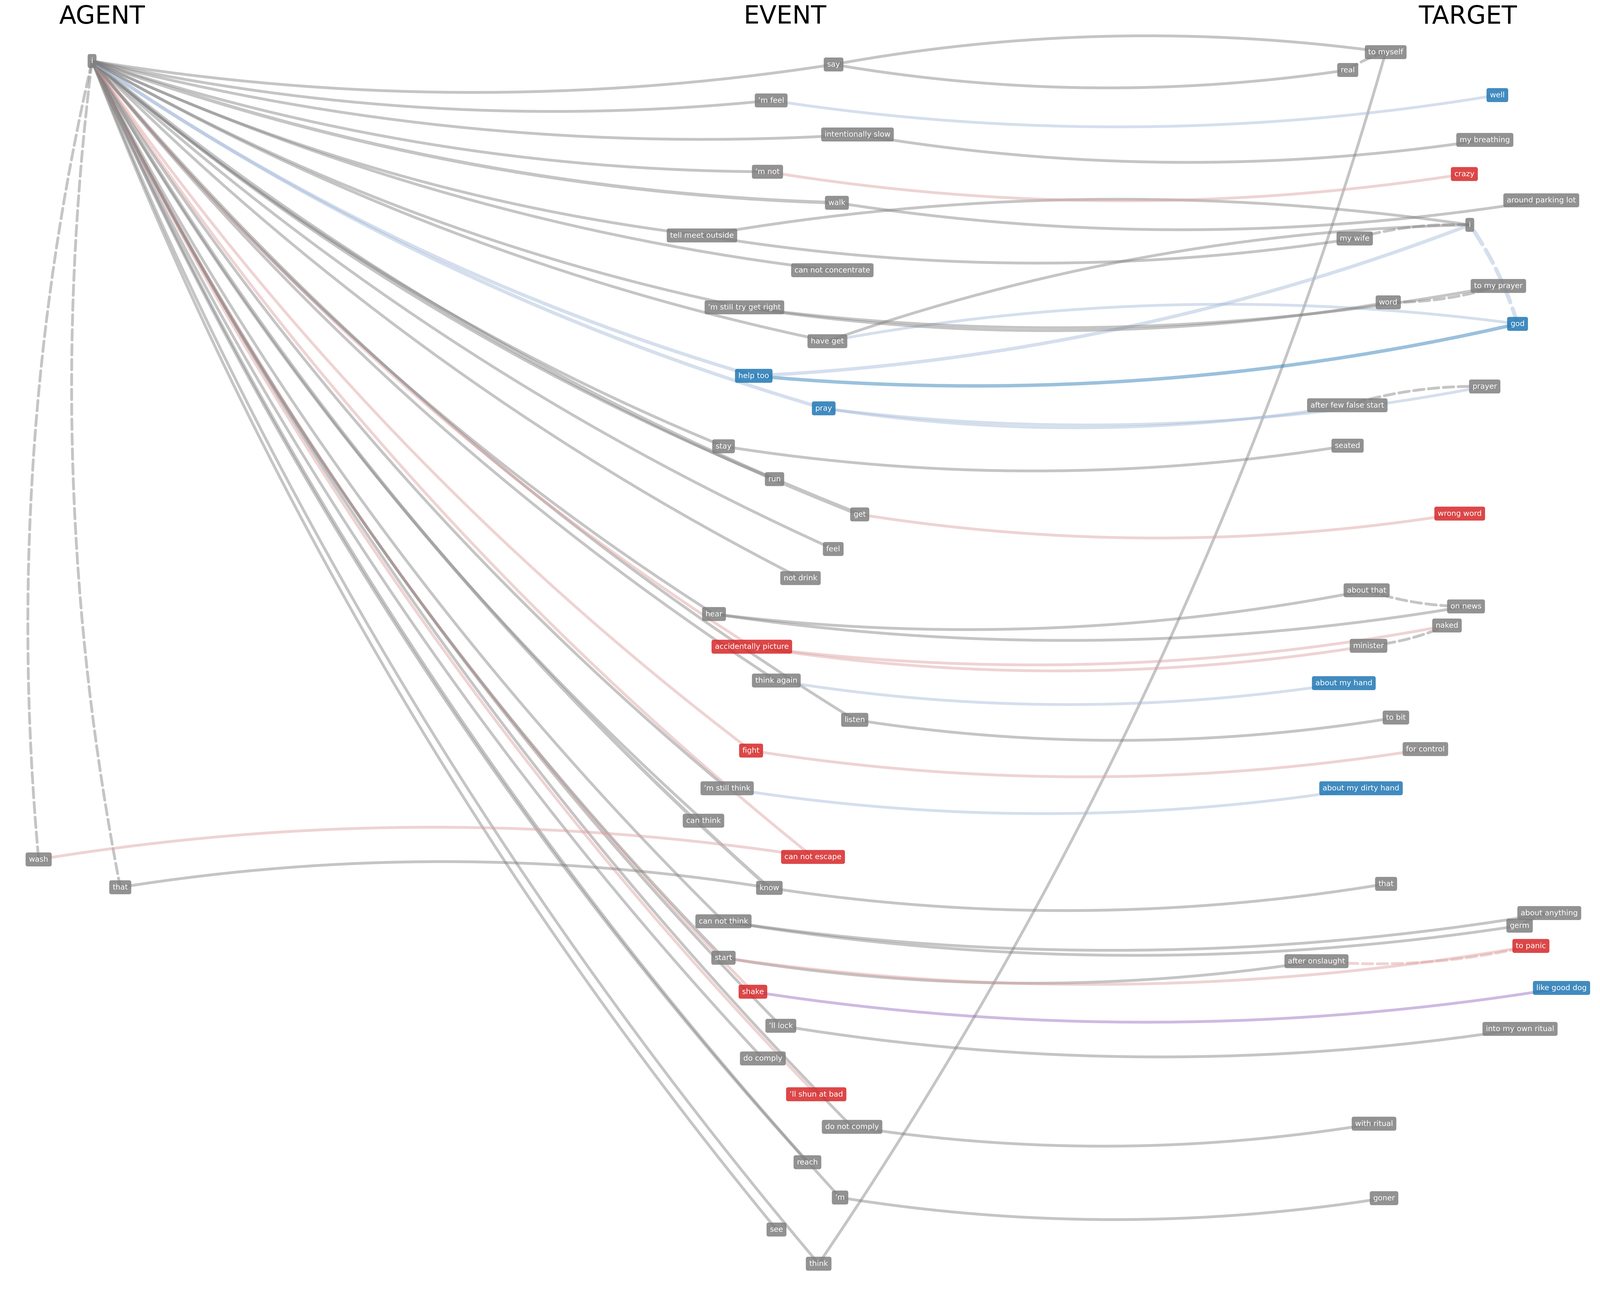
\includegraphics[width=\textwidth]{figures/tea_network_OCD_I.png}
\caption{TEA network of OCD narratives filtered by first-person subject (``I''), generated with \citeauthor{franchini2026tea}'s \texttt{plot\_svo\_graph}. Three-column layout: AGENT (left), EVENT (center), TARGET (right). Node color indicates VADER sentiment valence (blue = positive, red = negative, gray = neutral).}
\label{fig:tea_network}
\end{figure}

\begin{figure}[t]
\centering
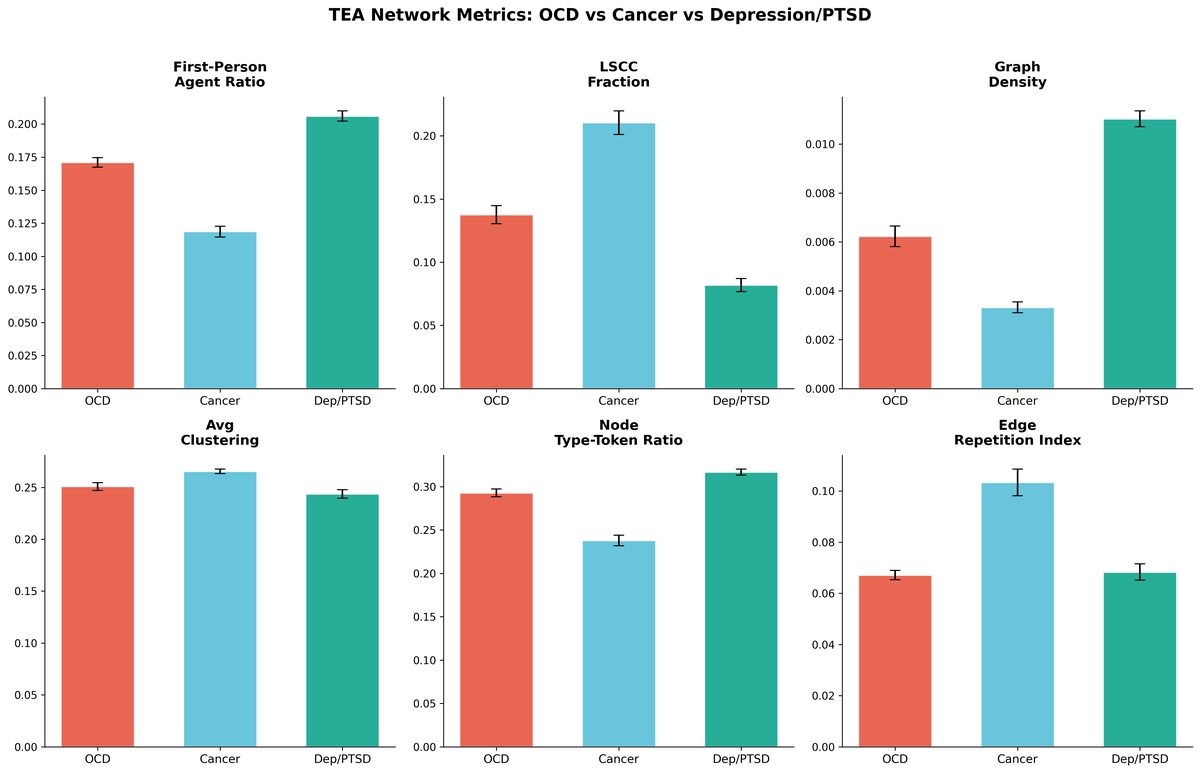
\includegraphics[width=\textwidth]{figures/tea_metrics_comparison.png}
\caption{TEA network metrics across three groups (mean $\pm$ SE). OCD narratives have a higher first-person agent ratio than cancer ($g = +1.37$) but lower than depression/PTSD ($g = -0.45$).}
\label{fig:tea_metrics}
\end{figure}

\begin{figure}[t]
\centering
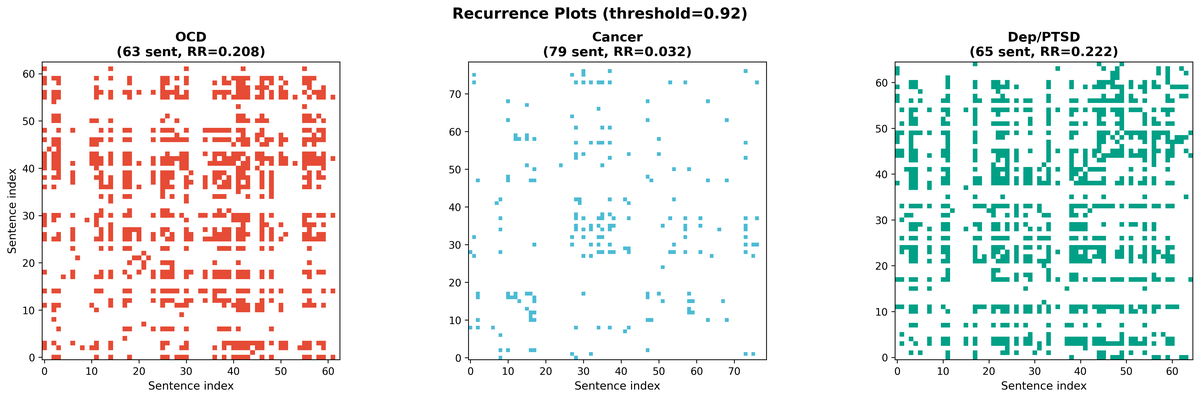
\includegraphics[width=\textwidth]{figures/recurrence_plots.png}
\caption{Recurrence plots for representative texts from each group (cosine similarity threshold $= 0.92$). Each dot marks a sentence pair above the threshold. OCD (left) shows dense, structured recurrence; Cancer (center) shows sparse recurrence; Depression/PTSD (right) shows the densest recurrence with large connected blocks.}
\label{fig:recurrence}
\end{figure}

\begin{figure}[t]
\centering
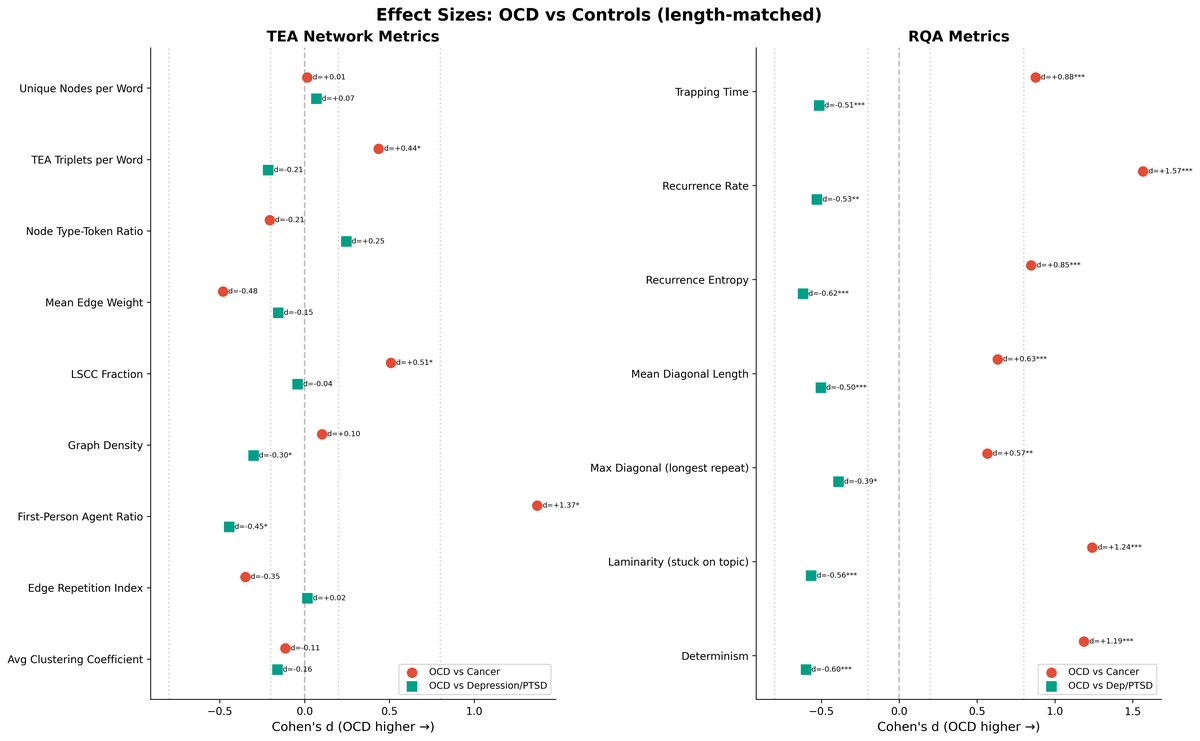
\includegraphics[width=\textwidth]{figures/effect_sizes_forest.png}
\caption{Forest plot of Hedges' $g$ for all length-matched comparisons. Left: TEA metrics. Right: RQA metrics. Red = OCD vs.\ Cancer; green = OCD vs.\ Depression/PTSD. Asterisks mark $p_\mathrm{BH} < .05$.}
\label{fig:forest}
\end{figure}

\begin{figure}[t]
\centering
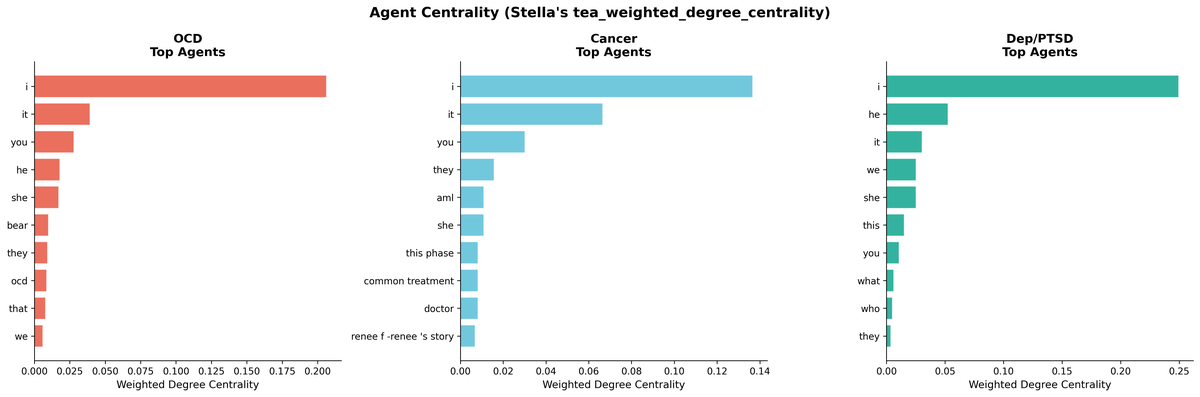
\includegraphics[width=\textwidth]{figures/top_agents_centrality.png}
\caption{Top 10 Agent nodes by weighted degree centrality for each corpus. ``I'' dominates all three corpora but with different relative centrality.}
\label{fig:centrality}
\end{figure}

\begin{figure}[t]
\centering
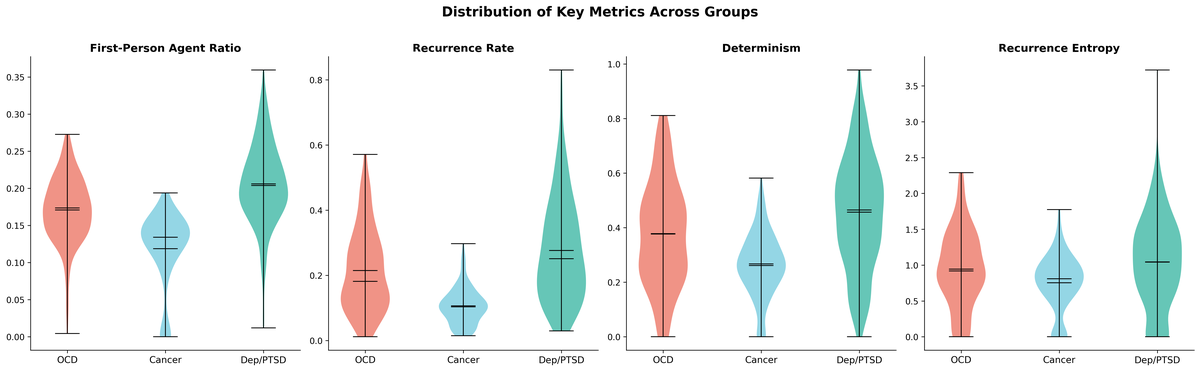
\includegraphics[width=\textwidth]{figures/violin_plots.png}
\caption{Distribution of four key metrics across groups: First-Person Agent Ratio (TEA), Recurrence Rate, Determinism, and Recurrence Entropy (RQA). OCD (red) falls between Cancer (blue) and Depression/PTSD (green) in all four panels.}
\label{fig:violin}
\end{figure}

% =====================================================================
\section{Discussion}

\subsection{The Gradient and Its Limits}

The main result is that OCD personal narratives sit between physical illness narratives and affective disorder narratives on two independently measured dimensions: self-focused agency (TEA) and thematic recurrence (RQA). After BH correction, 16 of 19 significant effects survived, with no contradictions among the non-significant metrics.

However, the three corpora differ not only in disorder type but also in platform (blog vs.\ interview site vs.\ Reddit), genre (unsolicited essay vs.\ edited transcript vs.\ social media post), editorial curation, and the narrators' likely relationship to their condition (OCD recovery stories vs.\ active-distress Reddit posts). These confounds limit the degree to which the gradient can be attributed to disorder type alone.

Several of the confounds could produce the observed pattern independently. Reddit posts tend to be more self-focused than blog posts regardless of clinical content, a pattern documented in computer-mediated communication research. Interview transcripts that have been professionally edited may show reduced repetitiveness compared to unedited personal writing. And narrators describing past recovery may use less self-focused, less repetitive language than those in active distress, independently of diagnosis.

We therefore interpret the gradient as a \emph{descriptive pattern in these corpora} that is consistent with, but not uniquely predicted by, disorder-specific cognitive models. Establishing whether the gradient survives within a single platform (e.g., comparing OCD, depression, and cancer communities on Reddit alone) would considerably strengthen the clinical interpretation.

\subsection{Depression vs.\ PTSD: A Differential Pattern}

Separating the two subreddits revealed a split. The self-focus gradient was driven primarily by depression: r/depression posters had higher first-person agent ratios than OCD narrators ($g = -0.72$), while r/ptsd posters did not differ significantly ($g = -0.32$). Depression and PTSD themselves differed on self-focus ($g = +0.47$). This is consistent with the self-focus literature, which has more consistently linked first-person pronoun use to depression than to PTSD \citep{rude2004}.

The thematic recurrence gradient, by contrast, appeared for both conditions, with larger effects for depression. RQA seems to tap a dimension, repetitive cognitive processing, that is elevated across affective conditions more broadly, while the self-focus metric is more specifically tied to depression.

\subsection{Self-Focus as Agentive Self-Monitoring}

TEA networks provide a view of self-focus that goes beyond counting pronouns. A high first-person agent ratio means that ``I'' fills the Agent slot, the grammatical position of the doer. The large effect ($g = +1.37$) between OCD and cancer tells us that OCD narrators cast themselves as agents far more often, directing actions at internal targets (thoughts, feelings, rituals) rather than recounting external events.

The effect sizes are lopsided: OCD is far from cancer ($g = +1.37$) but close to the depression/PTSD group ($g = -0.45$). On a linear scale, OCD falls roughly three-quarters of the way from cancer toward depression, meaning its self-focus is high in absolute terms and only moderately below affective-disorder levels. This is what one might expect from a condition defined by intense monitoring of one's own thoughts \citep{salkovskis1985}, though the platform confound (blog vs.\ Reddit) cannot be ruled out as a partial explanation.

The centrality profiles hint at a qualitative difference, though they rest on small samples and should be read as suggestive. In OCD narratives, ``I'' shares the agentive space with ``it'' (often referring to OCD as a separate entity) and ``you'' (addressing the reader or a generalized other). In depression/PTSD, ``I'' stands more alone, with a wider gap before the next agent. If this pattern holds in larger samples, it would be consistent with the ego-dystonic character of OCD, in which the disorder is experienced as an intruder rather than part of the self.

\subsection{Thematic Recurrence as a Repetitive-Thought Marker}

The RQA results provide the clearest differentiation. Effect sizes for OCD vs.\ Cancer range from $g = +0.57$ to $+1.57$ (medium to large), while those for OCD vs.\ Depression/PTSD range from $g = -0.39$ to $-0.62$ (small to medium). OCD narratives thus show roughly twice the thematic recurrence of cancer narratives but about three-quarters of the recurrence observed in depression/PTSD.

Looking at specific metrics: Laminarity in OCD ($M = 0.59$ vs.\ $0.37$ for cancer) indicates extended dwelling on single themes, consistent with the ``stuck'' quality of obsessional thinking. Determinism ($M = 0.41$ vs.\ $0.21$ for cancer) indicates that thematic revisits follow predictable sequences, consistent with the structured quality of compulsive thought. Both metrics are lower than in depression/PTSD (LAM $= 0.64$, DET $= 0.47$), where repetitive processing appears to produce broader thematic circularity. We note, however, that these metrics are computed on sentence-level embeddings (spaCy's 300-dimensional average word vectors), which are coarser than dedicated sentence transformers. Whether finer-grained embeddings would sharpen or alter the pattern remains untested.

\subsection{Implications}

We draw three implications, each limited by the caveats above.

First, the data provide language-based evidence consistent with treating OCD as distinct from both anxiety disorders and depression, in line with its reclassification in DSM-5 as part of the ``Obsessive-Compulsive and Related Disorders'' chapter \citep{apa2013}. The narrative signature of OCD is not simply ``more anxious than physical illness'' or ``less depressed than depression''; the combination of elevated-but-intermediate self-focus and structured recurrence points to a different cognitive pattern. This evidence is observational, drawn from convenience samples, and confounded with platform effects, so it supports the plausibility of the clinical distinction without constituting a direct test.

Second, the three-group design shows that metrics which look diagnostic in a binary comparison may reflect more general mental-health effects. The large first-person ratio difference between OCD and cancer ($g = +1.37$) could suggest self-focus as an OCD-specific marker, but the comparison with depression/PTSD ($g = -0.45$) shows that self-focus is elevated relative to physical illness but \emph{reduced} relative to other mental health conditions. Binary designs would miss this.

Third, Laminarity and Determinism from the RQA analysis appear to track meaningful variation in repetitive thought. The graded Cancer $<$ OCD $<$ Depression/PTSD ordering is what one would predict from existing theories of repetitive cognition across these conditions, though how much of the gradient comes from disorder type, how much from distress level, and how much from platform norms is still open.

\subsection{Limitations}

\paragraph{Platform and genre confounds.}
The three corpora come from different platforms with different genres, editorial practices, and audience norms. This is the study's most important limitation. Length matching addresses word-count confounds, but genre and platform differences in register, self-disclosure norms, and editorial intervention may independently affect the linguistic features we measured. A within-platform replication (e.g., comparing OCD, depression, and cancer communities on Reddit alone) would help isolate disorder-related variation from platform effects.

\paragraph{Recovery bias.}
The OCD corpus comes from a recovery-focused blog, meaning narrators are likely in remission or actively recovering. The depression/PTSD posts come from support-seeking communities and likely reflect more active distress. This confound could partially explain the gradient: lower recurrence and self-focus in OCD might partly reflect recovery stage rather than disorder type. Future studies should control for self-reported recovery status or symptom severity.

\paragraph{Unverified diagnoses.}
No clinical diagnoses were available for any group. OCD stories were posted on a dedicated recovery platform, and depression/PTSD posts came from disorder-specific subreddits, but diagnostic status is unverified.

\paragraph{OCD subtype heterogeneity.}
OCD is a heterogeneous condition with distinct symptom dimensions (contamination, checking, symmetry, intrusive thoughts). Different subtypes might produce different narrative patterns. The present study treats OCD as a single group; subtype-level analyses would require clinician-rated or self-reported subtype information.

\paragraph{NLP pipeline.}
The TEA extraction pipeline used spaCy's \texttt{en\_core\_web\_lg}, a statistical model rather than the transformer model recommended by the library for highest accuracy. The coreference resolution module was spaCy's \texttt{neuralcoref} component. For informal text (blog posts, Reddit), transformer-based models outperform statistical models on dependency parsing by 2--4\% UAS; however, SVO extraction rates were comparable across groups (0.47--0.52 triplets per word), suggesting that any parsing noise is distributed rather than systematically biased. RQA used spaCy's 300-dimensional average word vectors as sentence embeddings, which are coarser than dedicated sentence transformers (e.g., all-MiniLM-L6-v2). Whether sentence-transformer embeddings would alter the pattern is an open question.

\paragraph{Threshold sensitivity.}
The RQA recurrence threshold (0.923) was calibrated on a pooled sample. We did not run a formal sensitivity analysis across multiple thresholds; the robustness of the gradient to threshold choice remains to be established.

\paragraph{No healthy baseline.}
All three groups represent illness narratives. Without a non-illness comparison (e.g., personal narratives about hobbies or travel), we cannot determine whether the cancer end of the gradient represents ``normal'' narrative structure or its own clinical pattern.

% =====================================================================
\section{Conclusion}

OCD personal narratives occupy an intermediate position between cancer and depression/PTSD narratives on both self-focused agency (TEA networks) and thematic recurrence (RQA). After Benjamini-Hochberg correction, 16 of 19 originally significant effects survived, and the Cancer $<$ OCD $<$ Depression/PTSD ordering held for every surviving metric. Supplementary analyses showed that the self-focus gradient was driven primarily by the depression subgroup ($g = -0.72$) rather than PTSD ($g = -0.32$, n.s.), while the recurrence gradient generalized more broadly.

This pattern fits intrusion-driven models of obsessive cognition, but platform, genre, and recovery-stage confounds limit what can be concluded about causes. The study is best read as a methodological demonstration, showing how TEA networks and RQA can characterize illness-narrative structure, and as a descriptive finding that calls for within-platform replication. That two independent methods converge on the same ordering, despite their very different analytical logic, is the strongest reason to think the gradient reflects something real about these texts, whether its origin is cognitive, social, or some mix of both.

% =====================================================================
\section*{Data and Code Availability}

Analysis scripts and figure generation code are available at \url{https://github.com/Jacoposchenetti/Psychiatric_text}. The OCD corpus was collected from theocdstories.com, the cancer corpus from thepatientstory.com, and the depression/PTSD corpus from the HuggingFace dataset \texttt{solomonk/reddit\_mental\_health\_posts}. TEA networks were extracted with the TEA\_Networks library (\url{https://github.com/MassimoStel/TEA_Networks}, version 0.3.1).

% =====================================================================
\bibliography{references}

\end{document}
